% VUT FIT MITAI
% GAL 2020/2021
% Project: Topic 38 - Graph Radio Coloring Parallelization
% Authors: Vladimir Dusek, Patrik Goldschmidt

%%%%%%%%%%%%%%%%%%%%%%%%%%%%%%%%%%%%%%%%%%%%%%%%%%%%%%%%%%%%%%%%%%

\documentclass[11pt,xcolor=pdflatex]{beamer}
\usepackage{newcent}
\usepackage[utf8]{inputenc}
\usepackage[czech]{babel}
\usepackage{hyperref}
\usepackage{fancyvrb}
\usepackage{appendixnumberbeamer}
\usepackage{caption}
\usepackage{subcaption}
\usepackage{listings}

\usetheme{FIT}

\newcommand\myheading[1]{%
  \par\bigskip
  {\Large#1}\par\smallskip}

% Path for figures
\graphicspath{{images/}}

%%%%%%%%%%%%%%%%%%%%%%%%%%%%%%%%%%%%%%%%%%%%%%%%%%%%%%%%%%%%%%%%%%

\title[]{Topic 38 -- Graph Radio Coloring Parallelization}

\author[]{Patrik Goldschmidt, Vladimír Dušek}

\institute[]{Brno University of Technology, Faculty of Information Technology \\
Božetěchova 1/2. 612 66 Brno - Královo Pole, Czech Republic}

\date{17. December 2020}

%%%%%%%%%%%%%%%%%%%%%%%%%%%%%%%%%%%%%%%%%%%%%%%%%%%%%%%%%%%%%%%%%%

\begin{document}

\frame[plain]{\titlepage}

%%%%%%%%%%%%%%%%%%%%%%%%%%%%%%%%%%%%%%%%%%%%%%%%%%%%%%%%%%%%%%%%%%

\begin{frame}\frametitle{Graph Radio Coloring}

\begin{figure}[H]
    \begin{figure}[t]
        \centering
        \begin{subfigure}{.49\textwidth}
           \centering
           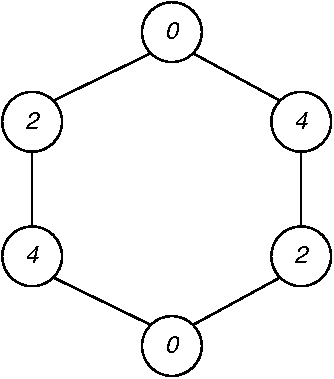
\includegraphics[width=0.7\linewidth]{circle_radiocolor.pdf}
           \caption{6-cycle graph radio coloring}
           \label{fig:circle_radiocolor}
        \end{subfigure}%
        \begin{subfigure}{.49\textwidth}
           \centering
           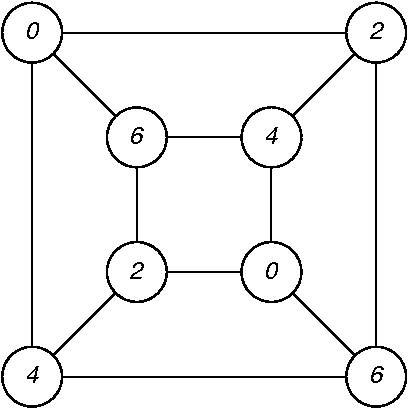
\includegraphics[width=0.75\linewidth]{cube_radiocolor.pdf}
           \caption{3-dimensional cube graph radio coloring}
           \label{fig:cube_radiocolor}
        \end{subfigure}
        \label{fig:radiocolor_example}
     \end{figure}
\end{figure}

\end{frame}

%%%%%%%%%%%%%%%%%%%%%%%%%%%%%%%%%%%%%%%%%%%%%%%%%%%%%%%%%%%%%%%%%%

\begin{frame}\frametitle{Formal Problem Definition}

Given an undirected graph $G = (V, E)$, the radiocoloring of $G$ is a mapping $f: V \rightarrow N$, such that $\forall v,u \in V: |f(u) - f(v)| \geq k + 1 - d(u,v)$, where $d(u,v)$ is a distance between $u$ and $v$ in $G$.

\end{frame}

%%%%%%%%%%%%%%%%%%%%%%%%%%%%%%%%%%%%%%%%%%%%%%%%%%%%%%%%%%%%%%%%%%

\begin{frame}[fragile]\frametitle{Sequential algorithm 1/2}

\begin{lstlisting}
# Step 1)
dist_matrix = floyd_warshall(adj_matrix)

C = Matrix(n, n)

# Step 2)
for i in (0 ... n):
    for j in (0 ... n):
        C[i][j] = max(k+1 - dist_matrix[i][j], 0)
    C[i][i] = INF

labels = [0, INF, INF, ...]
last = 0
\end{lstlisting}

\end{frame}

%%%%%%%%%%%%%%%%%%%%%%%%%%%%%%%%%%%%%%%%%%%%%%%%%%%%%%%%%%%%%%%%%%

\begin{frame}[fragile]\frametitle{Sequential algorithm 2/2}

\begin{lstlisting}
# Step 3)
repeat(n - 1):
    min_label = INF
    for j in (0 ... n):
        if min_label > C[last][j]:
            min_label = C[last][j]
            p = j
    for j in (0 ... n):
        C[p][j] += min_label
    for j in (0 ... n):
        if C[p][j] < C[last][j]:
            C[p][j] = C[last][j]
    labels[p] = min_label
    last = p
\end{lstlisting}

\end{frame}

%%%%%%%%%%%%%%%%%%%%%%%%%%%%%%%%%%%%%%%%%%%%%%%%%%%%%%%%%%%%%%%%%%

\begin{frame}\frametitle{Parallel algorithm}

\begin{itemize}
   \item Largest-degree first
   \item Algorithm
   \begin{itemize}
      \item Sort the vertices in descending order by their degree.
      \item Compute distance 2 binary matrix.
      \item Initialize a $n$ x $2n - 1$ binary matrix \emph{''forbidden``} ($O(n^2)$).
      \item Find the smallest non-conflicting color, assign it and update forbidden matrix.
   \end{itemize}
\end{itemize}

$$\textrm{DTIME} \approx O(n^2) + O(n \log n) + O(n^3) + O(n^3) \approx O(n^3)$$
\vspace{-3.5em}

$$\textrm{DTIME}_n \approx O(n) + O(\log n) + O(n^2) + O(n \log n) \approx O(n^2)$$

\end{frame}

%%%%%%%%%%%%%%%%%%%%%%%%%%%%%%%%%%%%%%%%%%%%%%%%%%%%%%%%%%%%%%%%%%

\begin{frame}\frametitle{Parallel algorithm - functionality}

\begin{figure}
   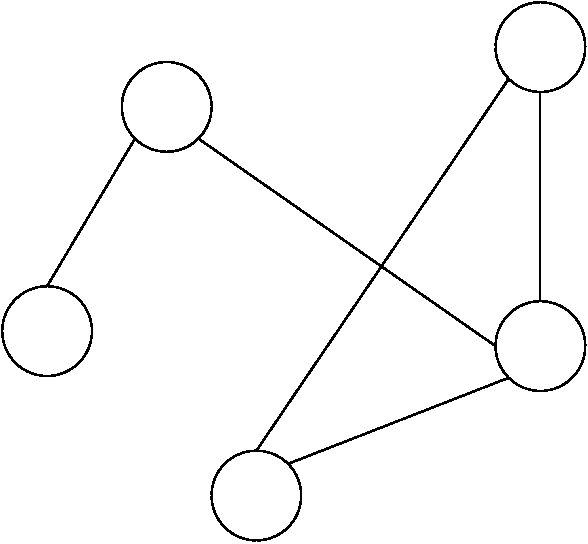
\includegraphics[width=0.6\linewidth]{graph_raw.pdf}
\end{figure}

\end{frame}

%%%%%%%%%%%%%%%%%%%%%%%%%%%%%%%%%%%%%%%%%%%%%%%%%%%%%%%%%%%%%%%%%%

\begin{frame}\frametitle{Parallel algorithm - functionality}

\begin{figure}
   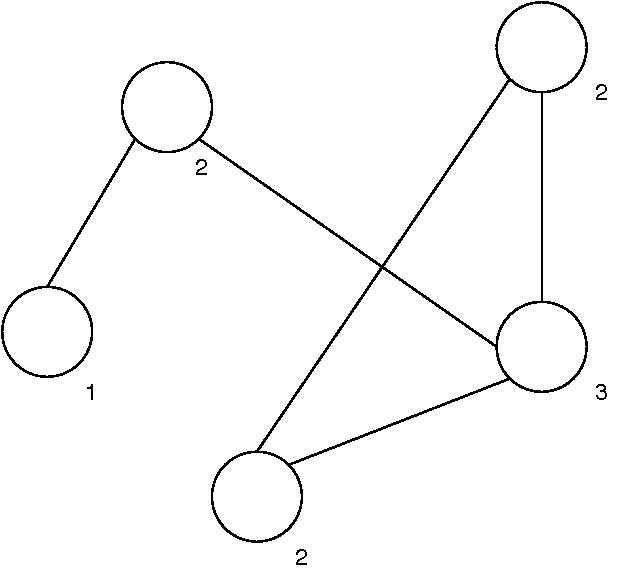
\includegraphics[width=0.6\linewidth]{graph_level.pdf}
\end{figure}

\end{frame}

%%%%%%%%%%%%%%%%%%%%%%%%%%%%%%%%%%%%%%%%%%%%%%%%%%%%%%%%%%%%%%%%%%

\begin{frame}\frametitle{Parallel algorithm - functionality}

\begin{figure}
   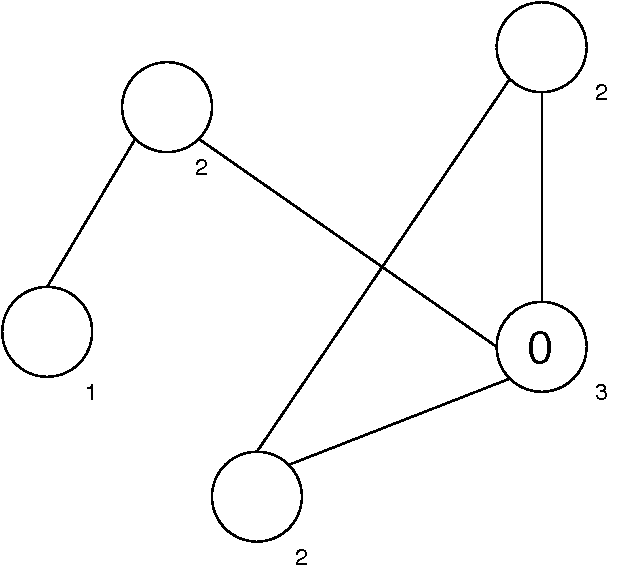
\includegraphics[width=0.6\linewidth]{graph_1colored.pdf}
\end{figure}

\end{frame}

%%%%%%%%%%%%%%%%%%%%%%%%%%%%%%%%%%%%%%%%%%%%%%%%%%%%%%%%%%%%%%%%%%

\begin{frame}\frametitle{Parallel algorithm - functionality}

\begin{figure}
   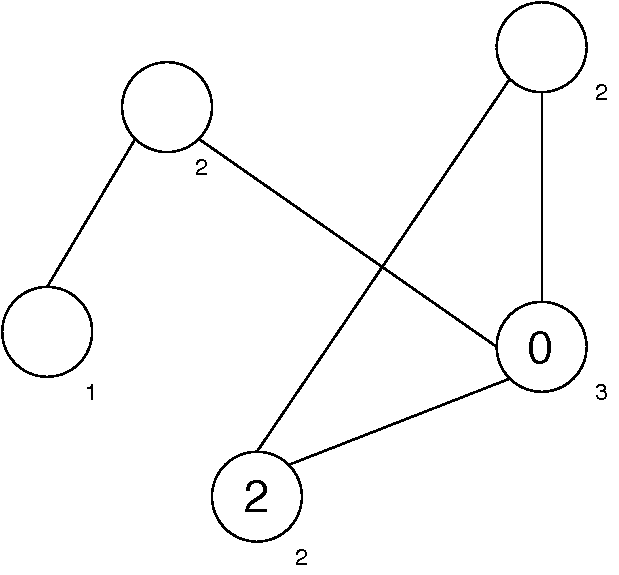
\includegraphics[width=0.6\linewidth]{graph_2colored.pdf}
\end{figure}

\end{frame}

%%%%%%%%%%%%%%%%%%%%%%%%%%%%%%%%%%%%%%%%%%%%%%%%%%%%%%%%%%%%%%%%%%

\begin{frame}\frametitle{Parallel algorithm - functionality}

\begin{figure}
   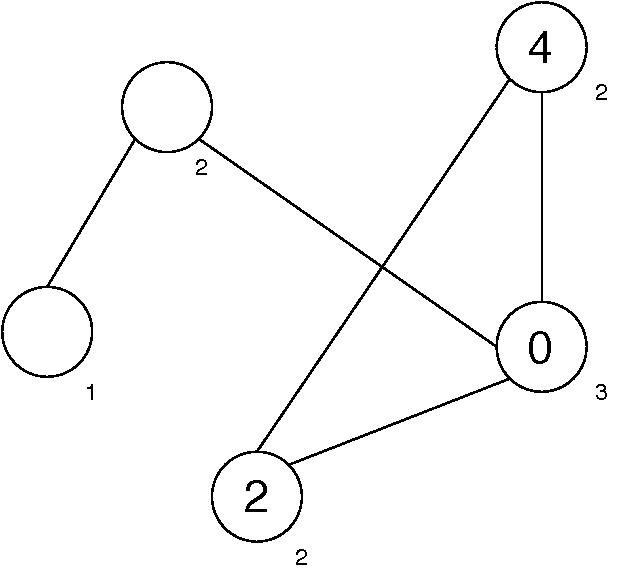
\includegraphics[width=0.6\linewidth]{graph_3colored.pdf}
\end{figure}

\end{frame}

%%%%%%%%%%%%%%%%%%%%%%%%%%%%%%%%%%%%%%%%%%%%%%%%%%%%%%%%%%%%%%%%%%

\begin{frame}\frametitle{Parallel algorithm - functionality}

\begin{figure}
   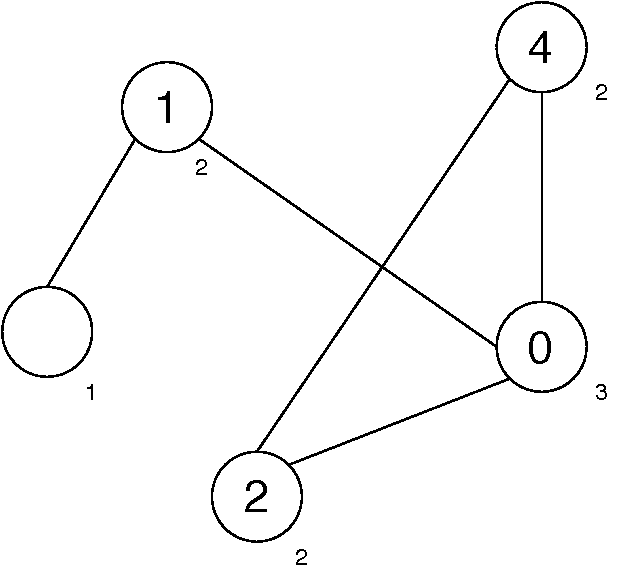
\includegraphics[width=0.6\linewidth]{graph_4colored.pdf}
\end{figure}

\end{frame}

%%%%%%%%%%%%%%%%%%%%%%%%%%%%%%%%%%%%%%%%%%%%%%%%%%%%%%%%%%%%%%%%%%

\begin{frame}\frametitle{Parallel algorithm - functionality}

\begin{figure}
   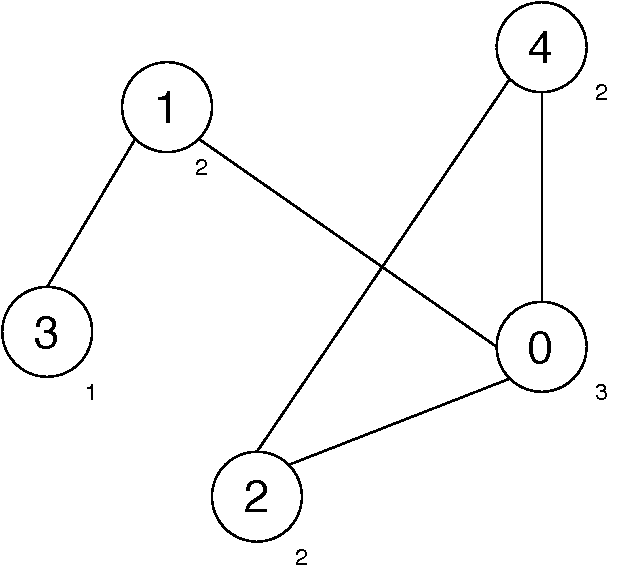
\includegraphics[width=0.6\linewidth]{graph_5colored.pdf}
\end{figure}

\end{frame}

%%%%%%%%%%%%%%%%%%%%%%%%%%%%%%%%%%%%%%%%%%%%%%%%%%%%%%%%%%%%%%%%%%

\begin{frame}\frametitle{Evaluation -- 1-threaded Algorithms Run}

\begin{figure}
   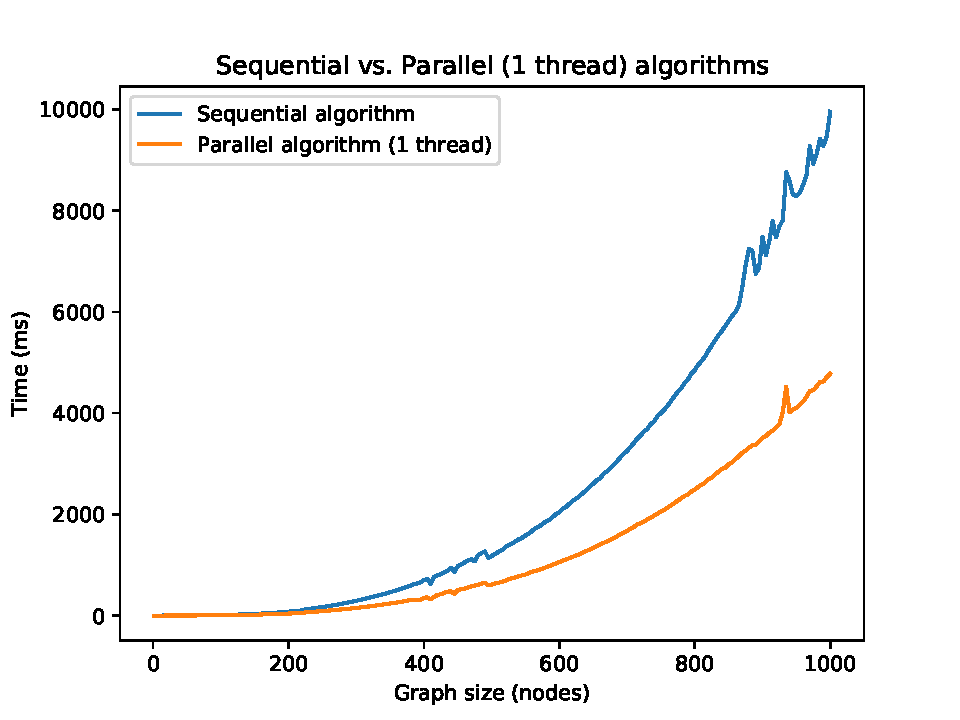
\includegraphics[width=0.9\linewidth]{comp_1thread.pdf}
\end{figure}

\end{frame}

%%%%%%%%%%%%%%%%%%%%%%%%%%%%%%%%%%%%%%%%%%%%%%%%%%%%%%%%%%%%%%%%%%

\begin{frame}\frametitle{Evaluation -- ``Optimized'' Parallel Variant}

\begin{figure}
   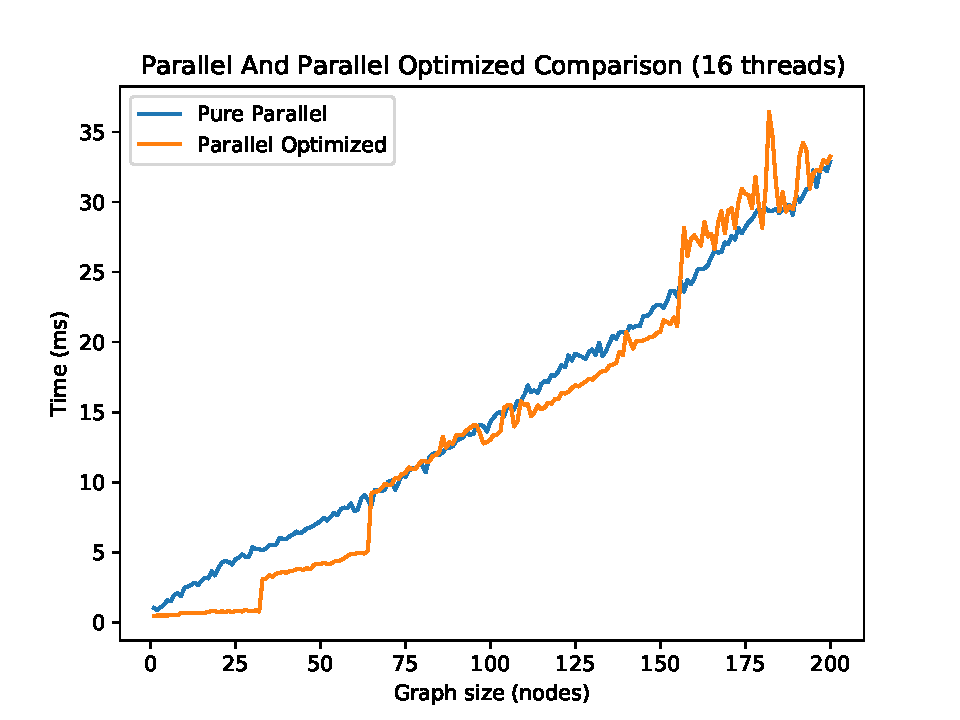
\includegraphics[width=\linewidth]{par_paropt16.pdf}
\end{figure}

\end{frame}

%%%%%%%%%%%%%%%%%%%%%%%%%%%%%%%%%%%%%%%%%%%%%%%%%%%%%%%%%%%%%%%%%%

\begin{frame}\frametitle{Evaluation -- Sequential vs. Parallel}

\begin{figure}
   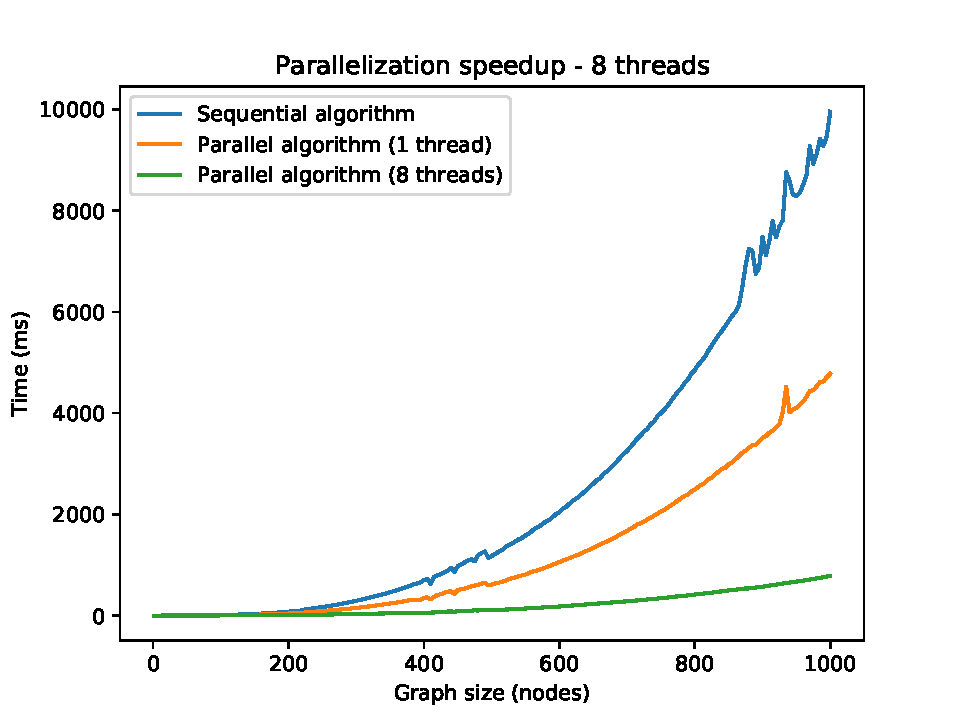
\includegraphics[width=\linewidth]{comp_8thread.pdf}
\end{figure}

\end{frame}

%%%%%%%%%%%%%%%%%%%%%%%%%%%%%%%%%%%%%%%%%%%%%%%%%%%%%%%%%%%%%%%%%%

\bluepage{Thank you for your attention}

%%%%%%%%%%%%%%%%%%%%%%%%%%%%%%%%%%%%%%%%%%%%%%%%%%%%%%%%%%%%%%%%%%

\end{document}
